
%\section{SICK Laser Scanner: Sensor Overview}

\section{Feature Detectors}

\subsection{Corner Detector}
\label{sec:corner_detector}
Corners are very common features in the indoor environment. They can be
easily detected using a laser range finder. Corners are generally
sparse, which makes the data association process more reliable. A single
observation of a corner is sufficient to completely define the pose of
the sensor. Using corners as features allows algorithms to be tested on
a clean simulation-like data, while still being realistic.


\begin{figure}[htbp]
  \centering
  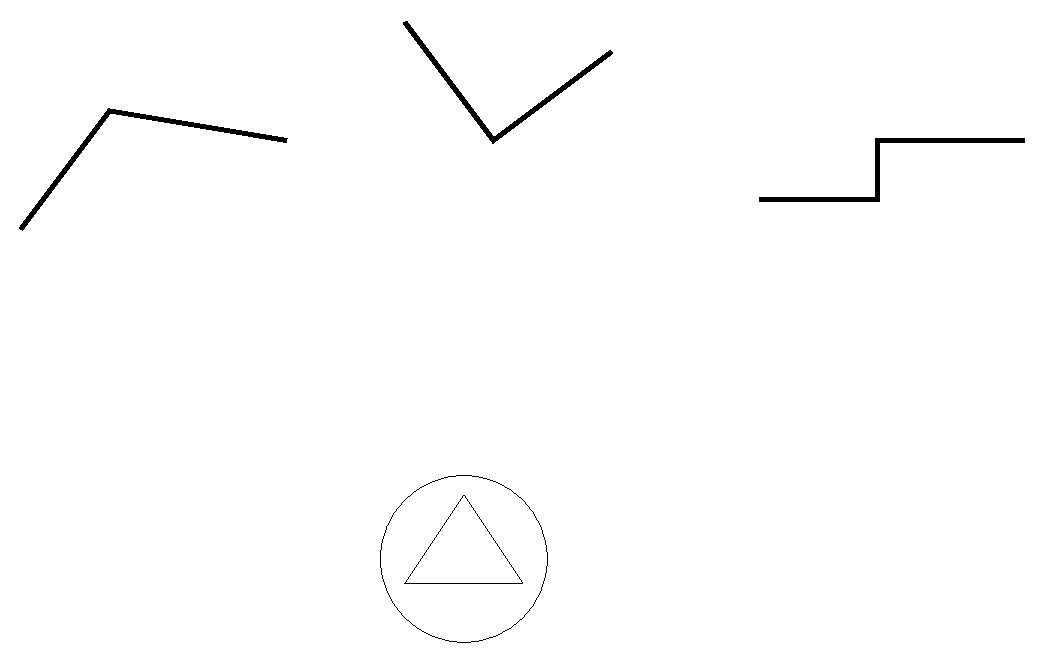
\includegraphics[width=5cm]{Pics/fig_corner_types}
  \caption[Types of corner features]{Corner types, from the left to the right: concave, convex,
  jump}
  \label{fig:corner_types}
\end{figure}

The corner detector algorithm distinguishes between three possible types
of corners: convex, concave and ``jump''. A ``jump'' corner is defined
as two parallel lines spaced a small distance apart. For example doors
in a hallway are classified by the algorithm as jumps.  It is possible
to detect a convex corner even when only one side of it is visible. Such
an observation is referred to as ``convex hidden''
corner. \refFigure{fig:corner_types} shows the different types of
corners.


\subsubsection{Algorithm}

The corner detector algorithm consists of two stages. During the first
stage the algorithm looks for regions in the laser scan that might
correspond to corners. During the second stage each corner hypotheses
is analysed more closely. Hypotheses that do not pass the tests are
discarded. Those that remain are classified to be either convex,
concave, jump or convex hidden corners.

\begin{figure}[htbp]
  \centering
  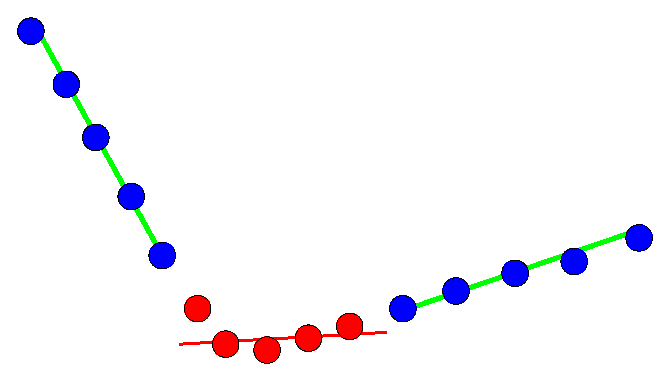
\includegraphics[width=5cm]{Pics/fig_corner_example}
  \caption{Trying to fit a line around the corner.}
  \label{fig:corner_example}
\end{figure}

During the first stage the algorithm looks at a narrow portion of the
laser scan (7 readings wide, that is only 3 degrees) and computes the
probability that this portion of the scan has been reflected from a
planar surface. This is achieved by fitting a line to the portion of
the laser scan and computing the average error. High error implies low
likelihood of the planar surface within the region. The algorithm starts
at the right most region of the laser scan and moves counter-clockwise
at one laser reading increment.

As the window slides along the planar region of the scan the error
remains low. However when the region includes corners and other
irregularities, the error increases significantly, and hence the line
quality drops, refer to \refFigure{fig:corner_example}. Regions where
the line quality falls from high to low are suspects for possible
corners, see \refFigure{fig:corner_scan_example_b}.

Some laser rays fail to reflect back to the sensor, either because
there is no obstacle in the sensor range, or due to the reflective
properties of the surface. If there are any ``no return'' rays within
the window, the quality of the line for this window is set to the
lowest. One can see in \refFigure{fig:corner_scan_example_c}, the
effect it has. While most hypothesis actually correspond to true
corners in the environment, there maybe false hypothesis arising from
sensor range limitations. However, the second stage of the algorithm
successfully removes any false hypothesis.
\refFigure{fig:corner_scan_example_d} demonstrates this point.

\begin{figure}[htbp]
  \centering
  
  \subfigure[Scan is taken from right to left,
  counterclockwise. ]
 {
    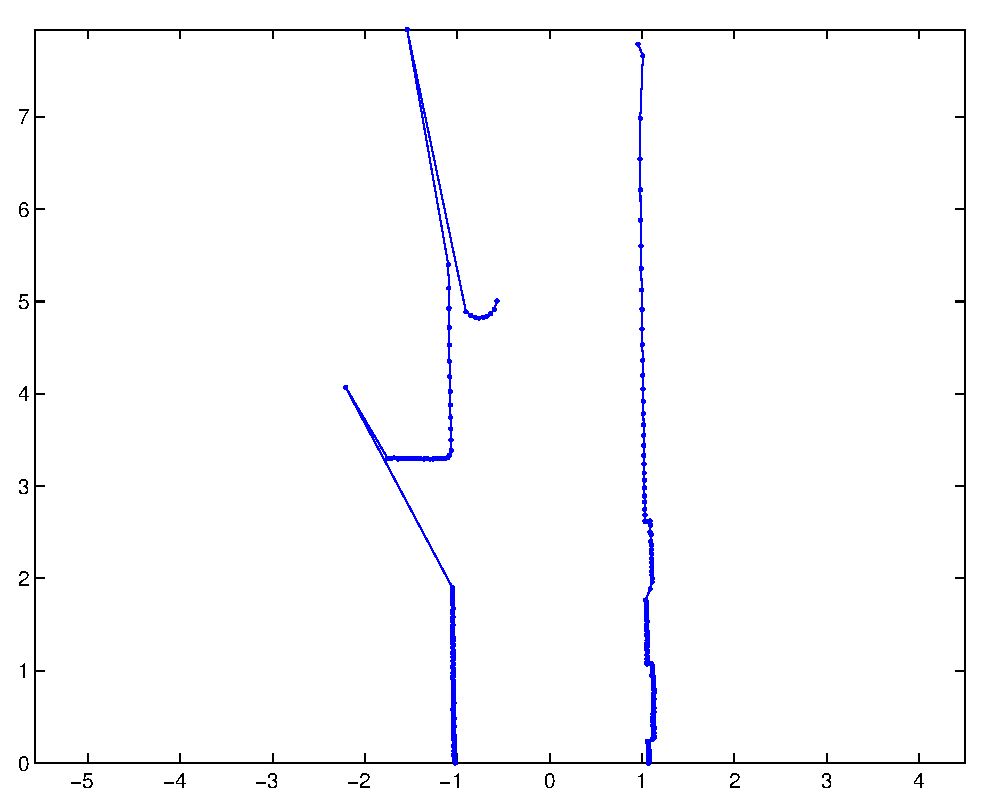
\includegraphics[width=6cm]{Pics/corner_scan_example_a}
  \label{fig:corner_scan_example_a}
} 
\subfigure[Negated total error squared is used as a measure of the
line quality. Horizontal line indicates good line threshold. Red lines
mark suspected corners.]{
  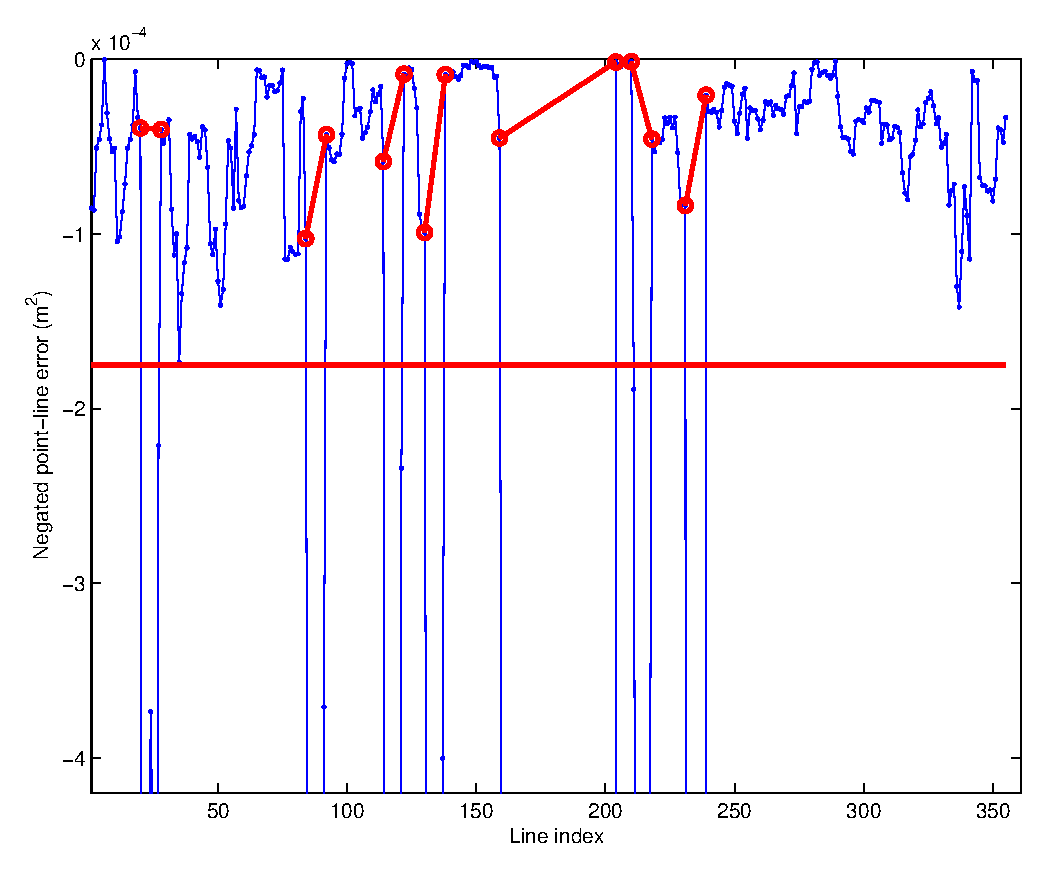
\includegraphics[width=6cm]{Pics/corner_scan_example_b}
  \label{fig:corner_scan_example_b}
}\\
\subfigure[Falls in line quality are suspect for corners. Circle
marks the beginning of the suspect region, square marks the end.]{
  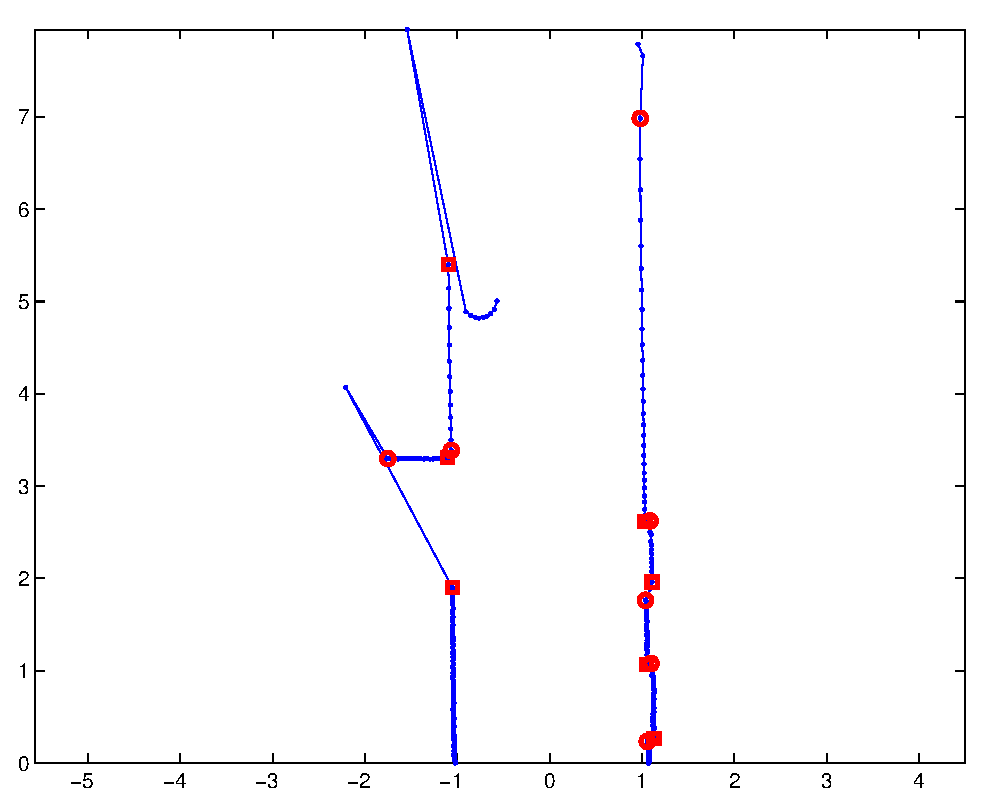
\includegraphics[width=6cm]{Pics/corner_scan_example_c}
  \label{fig:corner_scan_example_c}
}
\subfigure[Further tests confirm good corners and discard bad
ones. Corners are classified into several types.]{
  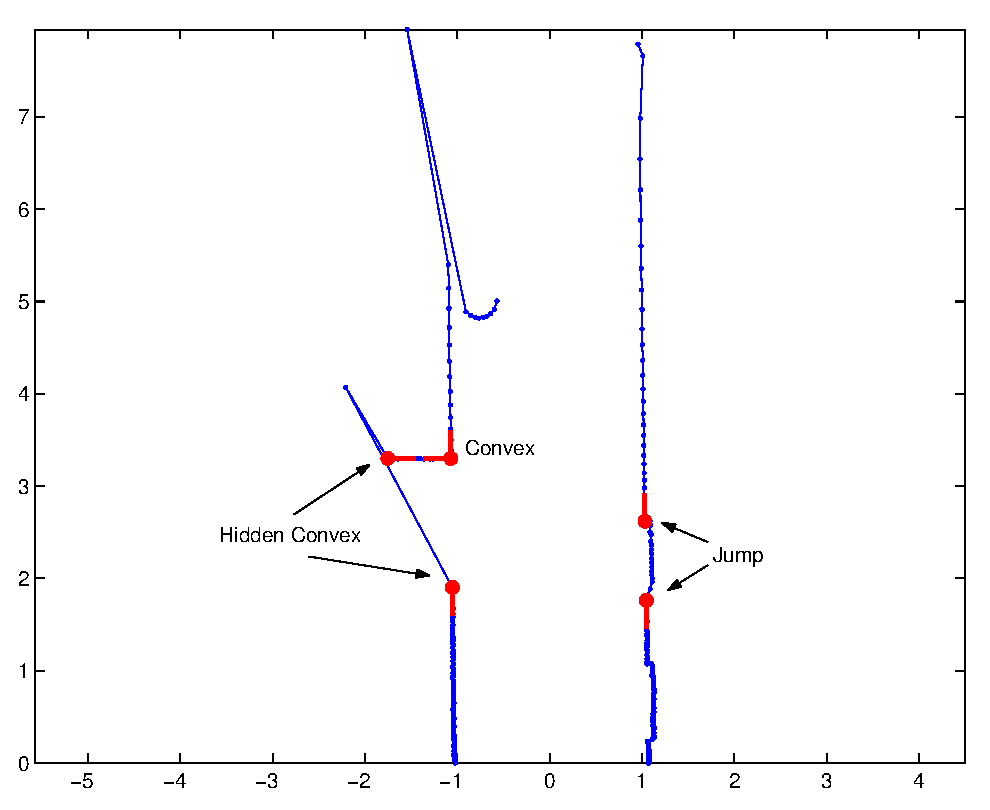
\includegraphics[width=6cm]{Pics/corner_scan_example_d}
  \label{fig:corner_scan_example_d}
}

\caption{Corner extraction from the laser scan.}
\end{figure}

The second stage of the corner detection algorithm classifies potential
corner observations as one of the: convex, concave, jump or convex
hidden corner, and discards those that do not fit either of the
models. Two intersecting lines to the left and to the right of the
suspected corner correspond to either convex or concave corner. Two
closely spaced collinear lines to the left and right of the corner
correspond to the ``jump'' corner. One line intersected by the laser
ray corresponds to the ``convex hidden'' corner.


\subsubsection{Uncertainty Representation}

A corner is considered to be a point landmark with additional
attributes. The additional attributes include the type of the corner
and the orientations of the corner arms. Overall there are four metric
parameters that define the corner: two parameters for the location and
two for the orientation of the corner arms. While it is possible to
compute the uncertainty directly from the laser readings, it is not
very obvious how to propagate the uncertainty of individual laser beams
through a line fitting process. In this work errors in the estimation
of the corner position and the orientation of the corner arms are
assumed to be independent zero mean Gaussians.

Observation of the corner location is expressed in polar coordinates.
Range and bearing measurements are assumed to be independent. 

Three standard deviations in the range measurement is set to 5 per
cent of the measured distance to the corner plus some constant. Three
standard deviations in the bearing measurement is set to 2 degrees.
Error in the estimate of the orientation of each arm is set to 3
degrees for three standard deviations. While this is a very simplistic
model of the uncertainty, in practice it performs surprisingly well.


\subsection{Tree Trunk Detector}

Locations of tree trunks were extracted from the laser data using the
matlab code available from the ACFR website \cite{VP_dataset}.


\section{Mapping}

This section describes the implementation of FastSLAM algorithm. It
defines the landmark update equations. Odometry models of vehicles
used in the experiment are also described.


\subsection{Point Landmarks}

Both trees and corners are treated as point landmarks. The extra
parameters, trunk diameter in the case of the tree landmark, and
orientation of the arms in the case of the corner landmark, are
assumed to be independent of the landmark position, and hence can be
estimated separately. The extra parameters are used for the data
association and for the computation of the probability of an
observation, given a landmark.

The point landmark is defined by its pose in the local reference
frame.

$$
{\bf x} = \left[ \begin{array}{c} x\\y \end{array} \right]
$$

The true state of the landmark is not known, the estimate of the
landmark state is maintained instead. The estimate of the landmark
state at time $k$ is $\hat{\bf x}_k$. The covariance for the landmark
state is also maintained and is denoted $P_k$.

The landmark state is related to the observation by the following equation
$$
  {\bf z} = h({\bf x},v) = \left[
\begin{array}{c}
\sqrt{(x-x_s)^2 + (y-y_s)^2}\\ \noalign{\medskip}
\tan^{-1} \frac{y-y_s}{x-x_s} + \theta_s
\end{array}
\right] + v
$$
here $x_s$, $y_s$ and $\theta_s$ denote the location and heading of
the sensor in the local reference frame and $v$ is the observation noise,
assumed to be zero mean Gaussian.

The Jacobian of partial derivatives of $h$ with respect to landmark
state is

$$
H_{[i,j]} = \frac{\partial h_{[i]}}{\partial {\bf x}_{[j]}}
             \left(\hat{\bf x}_k , 0 \right).
$$

For clarity lets define the estimate of the landmark location in the
sensor centric coordinate frame as $\hat{x}' = \hat{x} - x_s$ and
$\hat{y}' = \hat{y} - y_s$. The Jacobian above is then equal equal to:

$$
H = 
 \left[ \begin {array}{cc}
   \frac{\hat{x}'}{ \sqrt{\hat{x}'^2+\hat{y}'^2} } & 
   \frac{\hat{y}'}{ \sqrt{\hat{x}'^2+\hat{y}'^2} } \\ \noalign{\medskip}
   \frac{-\hat{y}'}{ \hat{x}'^2+\hat{y}'^2 } & 
   \frac{ \hat{x}'}{ \hat{x}'^2+\hat{y}'^2 }.
\end{array} \right] 
$$

The Jacobian of partial derivatives of $h$ with respect
to noise is also required by the EKF, in this case it is trivial

$$
V_{[i,j]} = \frac{\partial h_{[i]}}{\partial v_{[j]}}
             \left(\hat{\bf x}_k , 0 \right) = I.
$$

These Jacobians evaluated at the current state are used to update the
state of the landmark when a new observation becomes available.


\subsubsection{Observation Update}

Every time a landmark is observed, its pose estimate is updated to
take into account the new information. This update is performed using
the standard Extended Kalman filter equations.


\subsubsection{Genesis}

When an observation does not match any of the existing landmarks, a
new landmark is added to the map. A range and bearing observation is
converted into a Cartesian coordinate space. The covariance of the
landmark is computed from the covariance of the measurement using
first order Taylor series approximation.


\subsection{XR4000: Odometry Model}

The robotic platform used for the indoor experiment is an XR4000 robot
from Nomadic Technology. This robot has a holonomic drive system with
four wheels. Controllers on-board the robot integrate distance
travelled by each of the wheels to compute the location of the robot
in some global reference frame. This estimate is subject to drift
due to the accumulation of errors in the process of integration. It is
difficult to model such a system from the physical principles, instead
a simplified model is devised.

The state of the robot at time $k$ is its position and orientation in a
local reference frame

$$
\x{k}{}{} = \left[\begin{array}{c} 
    x_k \\ 
    y_k \\ 
    \theta_k
  \end{array}\right].
$$

Being a holonomic robot, the XR4000 can move in any direction and rotate
at the same time, just like an office chair. Control input \U{k} is
defined as an instantaneous translational and rotational velocity of the
robot at time $k$. Translational velocity is expressed in polar
coordinates $[v_k,\psi_k]^T$ in the robot centred frame. $\omega_k$ is a
rate of rotation of the robot centred frame relative to the reference
frame

$$
\U{k} = \Vector{v_k\\ \psi_k \\ \omega_k}.
$$

In the case of the XR4000, the state evolves according to the following
rule

$$
\x{k}{}{} = f(\x{k-1}{}{} ,\U{k-1}) = \x{k-1}{}{} + \Delta {\bf t}
\Vector{v_k\cos(\theta_{k-1} + \psi_{k-1})\\
v_k\sin(\theta_{k-1} + \psi_{k-1})\\
\omega_{k-1}}.
$$

Since \U{k} is not available directly it has to be derived from the
integrated robot poses returned from the on-board wheel controllers.
\U{k} is computed by the differentiation of the controller readings.

\begin{figure}[htbp]
  \centering

  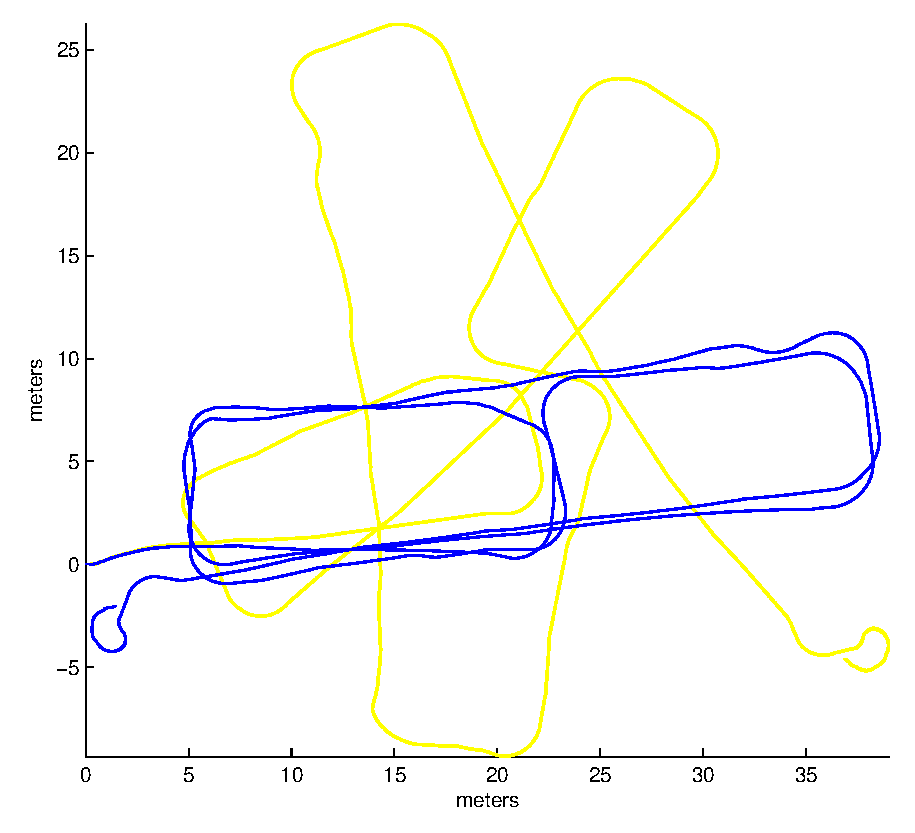
\includegraphics[width=10cm]{Pics/xr4000_raw_odo}
  
  \caption[XR4000 odometry bias]
     {XR4000 Odometry, before correcting for bias (light line)and after (dark line)}
  \label{fig:xr4000_raw_odo}
\end{figure}

{\bf Bias Correction}\\ The XR4000 used in this experiment has a
significant drift to the right, when travelling on a straight
line. Experiments revealed that, when the robot is instructed to travel
on a straight line forward, it actually follows an arc of 100 meter
radius, that corresponds to a rotation of $0.57^\circ$ to the right per
meter travelled. This bias is corrected by adjusting rotational velocity
$\omega_k$, and the heading of the translational velocity $\psi_k$
accordingly.

When the robot is travelling on a curve, the bias is likely to be
different, however no experiments were conducted to estimate it. It is
assumed to be equal to that of the straight line.


\subsection{Truck: Odometry Model}

An Ackerman model is used to model the odometry of the truck used to
collect the Victoria Park data set. Sensor input consists of the
velocity of the left rear wheel and the angle of the front
wheel. Velocity of the centre of the vehicle $v_c$ is computed from the
velocity of the left wheel $v_e$ using the following:

$$
v_c = \frac{v_e}{1 - \tan \alpha \frac{H}{L}}.
$$

The state of the truck is defined by

$$
\Vector{x_k\\y_k\\\theta_k} = f(\x{k}{}{},\U{k}) = 
\x{k}{}{} + v_c \Vector{\cos \theta_{k-1} \\ \sin
  \theta_{k-1} \\ \frac{\tan \alpha}{L}} \Delta T.
$$

In the above: L=2.83m - the distance between the front and rear axles,
H=0.76m - half the distance between the rear wheels. Truck coordinate
system is set at the middle of the rear axle with $x$ axis pointing
forward and $y$ axis pointing left. The laser sensor is mounted at 3.78m,
0.5m.

\subsection{Region Model: Indoors}

For the indoor experiment region extent was computed directly from the
laser scans. The first five scans are used to compute the free space in
front of the robot. This region defines the extent of the local map.
The occupancy grid is computed by a standard ray tracing algorithm. Any
uncertainty in the robot pose is ignored when building the occupancy
grid.

\subsection{Region Model: Victoria Park}

In outdoor environments free space dominates. It is therefore possible
to assign any region to the local map. A grid map with a resolution of
50cm is used. The initial map region is a rectangle aligned with the
robot heading direction. At the end of the mapping process the region
is trimmed, as shown in \refFigure{fig:initial_region_vision}. Trimmed
region is set to the intersection of the initial region and the region
formed by the convex hull of the map. When computing the convex hull
of the map any uncertainty in landmark estimates is ignored.

\begin{figure}[htbp]
  \centering
  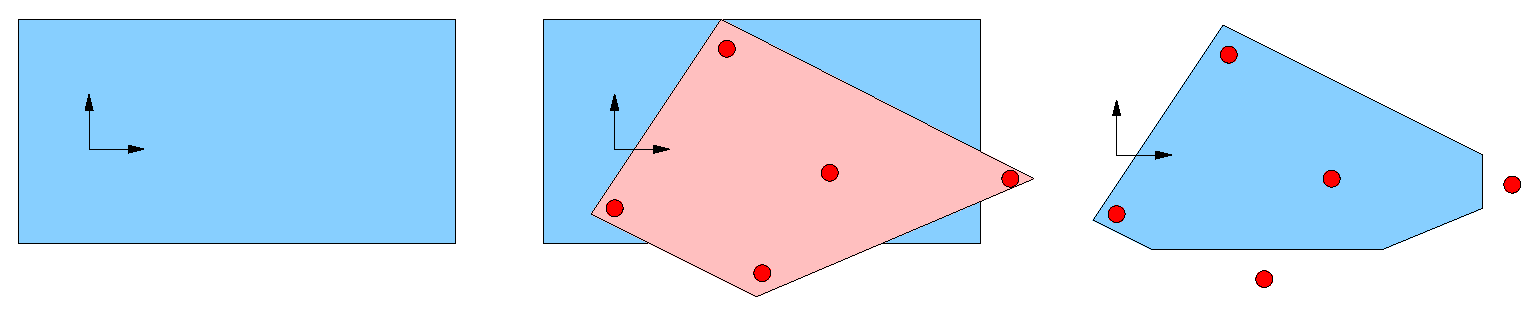
\includegraphics[width=14cm]{Pics/fig_convex_reg}
  \caption[Example of region evolution]
  {Example of region evolution: start with a polygon regions,
  after mapping is complete fit convex hull to the map, set region to
  the overlap between the initial region and the convex hull.}
  \label{fig:initial_region_vision}
\end{figure}

\section{Experiment Setup and Analysis}

Particle filters produce different output for the same input (it is
the nature of the filter). As a result, the performance of a particle
filter can not be judged based on just one execution of the
algorithm. 


%What quality measured can be used to judge the performance of a PF?
Traditionally a RMS (Root Mean Squared) distance from the estimate to
the true state is used to judge the quality of the PF. To use this
metric one needs to know the true state of the system. In the case of
a SLAM problem the path of the robot needs to be known. RMS is not a
very useful metric for the purposes of this thesis, since HTSLAM does
not produce a global estimate of the path. Even for global mapping
approaches this metric is of little use, since the RMS error is likely
to increase as the robot travels further away from the starting point.
High RMS error on the fringes of the map does not always suggest a bad
map, while even relatively low RMS error near the origin of the map
may indicate an inconsistent map.

Self-consistency is a more important measure of the quality of the
map, though it is harder to define and measure. In the ideal world the
definition can be simple: the map should contain only those landmarks
that exist in the environment and have been observed during the
experiment. All observations should be assigned to the correct
landmark. In real life experiments this condition will never hold.
Sensors do produce erroneous readings. Data association is often
ambiguous, especially in the environments where landmark density is
higher than the sensor uncertainty. Furthermore finding the true
correspondences between all landmarks and all observations is a
prohibitively laborious task.

\begin{figure}[htbp]
  \centering
  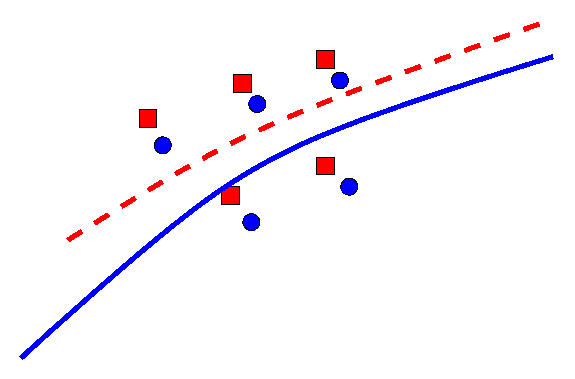
\includegraphics[width=5cm]{Pics/fig_inconsistent_map}
  \caption[Example of an inconsistent map]
  {Example of an inconsistent map. On a second pass through
    the region (dashed line), data association failed and the robot
    erroneously added new landmarks (squares).}
  \label{fig:inconsistent_map}
\end{figure}


The map self-consistency requirement needs to be relaxed to
accommodate for a realistic situation. In this work the following
definition is used: if the filter experiences systematic data
association errors, and diverges from the ground truth path, then the
map is considered to be inconsistent. \refFigure{fig:inconsistent_map}
shows an example of an inconsistent map. Errors such as these are easy
to spot for a human operator with a priori knowledge of the
environment.

The HTSLAM map is considered to be consistent if all local maps are
consistent, and if all relative map transformations are consistent.
Inconsistencies in relative local map poses can arise during loop
closing, when incorrect map correspondences are established.
Generally, inconsistent relative poses lead to inconsistent local
maps, and are therefore easy to detect. Failure to close the loop does
not result in the inconsistent map, however such a map provides less
information about the environment, and is therefore inferior to a
proper map.

\section {Results Indoors}

%Describe the environment.
Indoor experiments were performed on the third floor of the RSISE
building in ANU. A schematic of the environment is shown in
\refFigure{fig:rsise_level3_map}.

The HTSLAM algorithm was run 100 times on each data set. The map from
each run was classified as one of: consistent and proper (closed
loop), consistent but improper (failed to close the loop) or
inconsistent.

 
\begin{figure}[htbp]
  \centering
  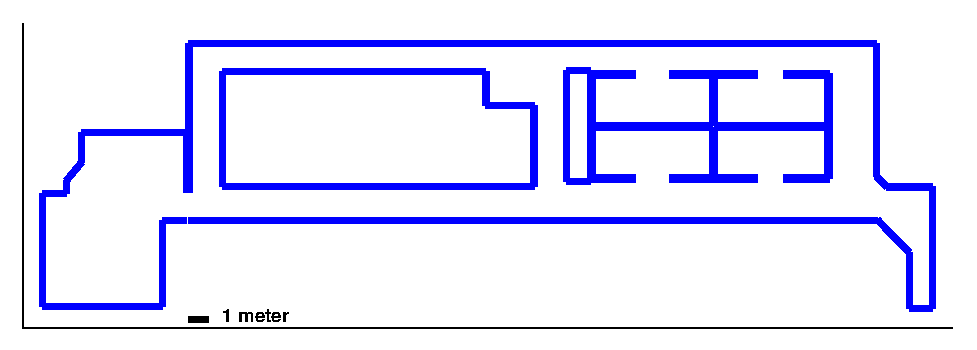
\includegraphics[width=13cm]{Pics/rsise_level3_map}
  \caption{Indoor environment: RSISE level 3.}
  \label{fig:rsise_level3_map}
\end{figure}

The same data set was processed with 100 and 300 particles. One
hundred runs, each with a different random seed, were taken to discard
the possibility of a ``lucky run''. All of the runs have produced
correct maps on this particular data set.

For each run HTSLAM produces one map for every particle. It is not
practical to plot the maps for each particle, instead a single sample
from the final distribution is displayed. There is no global reference
frame in HTSLAM, however for display purposes a robot starting pose was
used as a reference frame. All the local maps for a single particle
are plotted in that reference frame.

\refFigure{fig:corner_map_100p} shows one of the maps built with one
hundred particles. Local maps are projected into the reference frame
of the first map. Note that no post-processing was performed to align
the maps. \refFigure{fig:corner_map_300p} shows one of the maps
produced with 300 particles. The paths of all runs projected into the
reference frame of the first map are presented in
\refFigure{fig:corner_odo_all}. As expected, the path estimate differs
more between runs further from the origin.


\begin{figure}[htbp]
  \centering
  \subfigure[Projection of the HTSLAM map in the reference frame of map 1.]{
    \includegraphics[width=15cm]{Pics/corner_map_100p}
  }
  \subfigure[Topological path of the robot.]{
    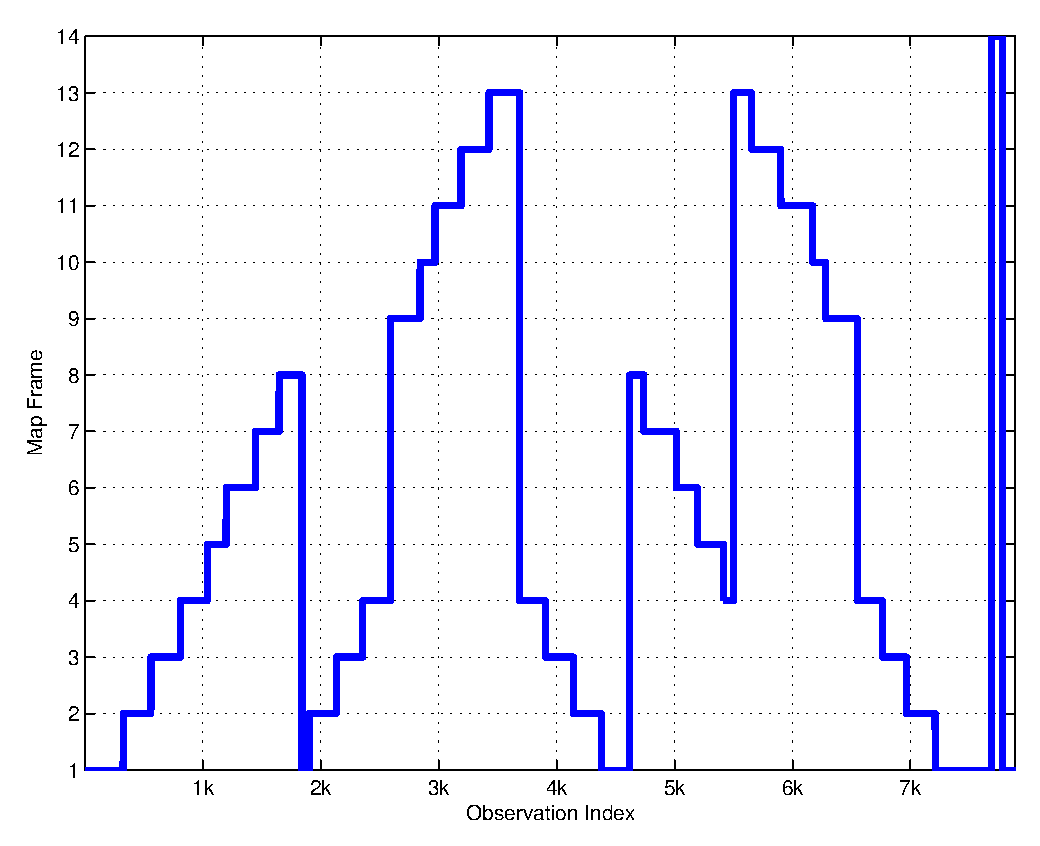
\includegraphics[width=10cm]{Pics/corner_odo_100p}
  }
  \caption{Laser indoors: Map of corners (100 particles)}
  \label{fig:corner_map_100p}
\end{figure}

\begin{figure}[htbp]
  \centering
  \subfigure[Projection of the HTSLAM map in the reference frame of map 1.]{
    \includegraphics[width=15cm]{Pics/corner_map_300p}
  }
  \subfigure[Topological path of the robot.]{
    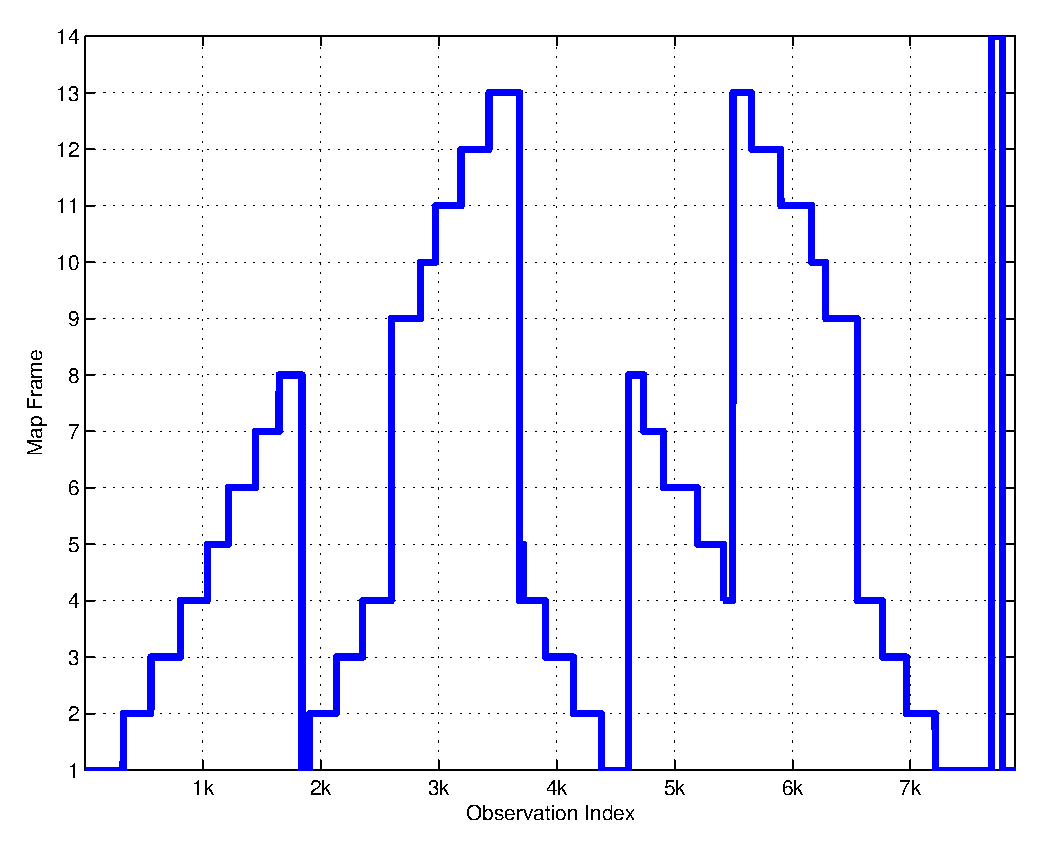
\includegraphics[width=10cm]{Pics/corner_odo_300p}
  }
  \caption{Laser indoors: Map of corners (300 particles)}
  \label{fig:corner_map_300p}
\end{figure}

\begin{figure}[htbp]
  \centering
  \subfigure[100 particles]{
    \includegraphics[width=15cm]{Pics/corner_odo_all_100p}
  }
  \subfigure[300 particles]{
    \includegraphics[width=15cm]{Pics/corner_odo_all_300p}
  }
  \caption{Laser indoors: Global Path over 100 test runs.}
  \label{fig:corner_odo_all}
\end{figure}


\subsection{Execution time}


\begin{figure}[htbp]
  \centering
  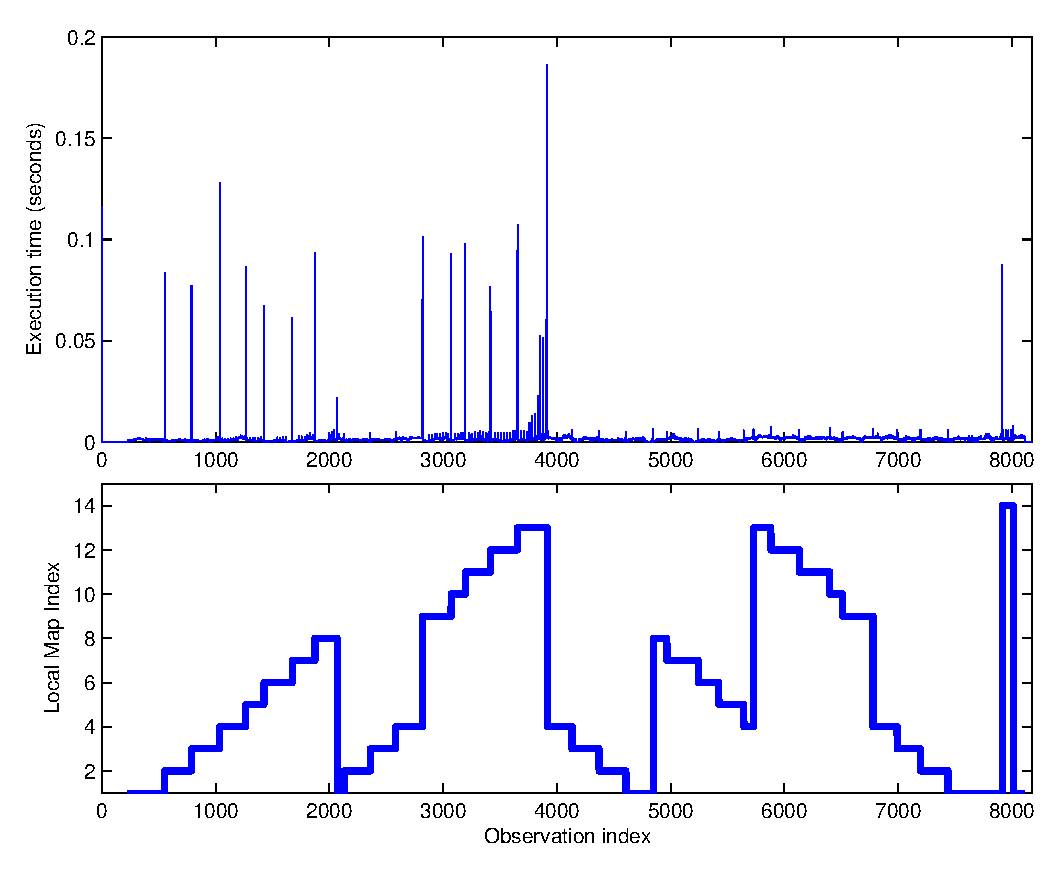
\includegraphics[width=15cm]{Pics/corners_execution_time}
  
  \caption{Laser indoors: Execution time 100 particles.}
%map 33
  \label{fig:corners_execution_time}
\end{figure}

\refFigure{fig:corners_execution_time} shows the plot of execution time
per laser reading for one of the runs (100 particles were used).  The
spikes in the execution time correspond to the creation of the new
region. Most of this time is spent computing the occupancy grid of the
region. It is possible to do this computation in the background, while
robot is still processing new observations. Note that the graph never
exceeds 0.2 seconds, which is the time between observations in case of
the SICK laser range finder. The algorithm runs faster than
real-time. An important thing to note is that computation time per
observation remains constant throughout the experiment. Even though
robot explores larger and larger area and the size of the map grows, the
time to process an observation remains roughly the same.


\section {Results Victoria Park}

The Victoria park data set has been processed in a similar manner to
the indoor data set: 100 randomised runs of 100 and 300
particles. While the majority of the runs have produced a correct map,
some have failed. Table~\ref{tab:results_victoria_park} shows the
proportion of successful runs for 100 and 300 particles.


\begin{table}[ht]
\center
\begin{tabular}{r|c|c|c}
Num. Particles & Consistent & Consistent but improper & Inconsistent\\
\hline
100 & 75  & 0 & 25 \\
300 & 93  & 0 & 7\\
\end{tabular}
\caption{Laser outdoors: Summary of the experiments on the Victoria Park data set.}
\label{tab:results_victoria_park}
\end{table}

The result for a run with 100 particles is quite disappointing - every
fourth execution of an algorithm failed to build a consistent
map. However when the number of particles is increased to 300 the
failure rate falls to 7 per cent. This a positive sign as it indicates
that most failures are probably due to insufficient number of particles
used. Manual inspection of the failed maps suggests that most of the
failures happen straight after a first transition in to a previously
mapped region. Better sampling strategy for the first transition might
improve the performance of the algorithm.

\refFigure{fig:trees_map_100p} and \refFigure{fig:trees_map_300p} show
an example of a correct map for 100 and 300 particles
respectively. \refFigure{fig:trees_odo_all} shows paths of all runs
projected in to the reference frame of the first map.


\begin{figure}[htbp]
  \centering
  \subfigure[Projection of the HTSLAM map in the reference frame of map 1.]{
    \includegraphics[width=15cm]{Pics/trees_map_100p}
  }
  \subfigure[Topological path of the robot.]{
    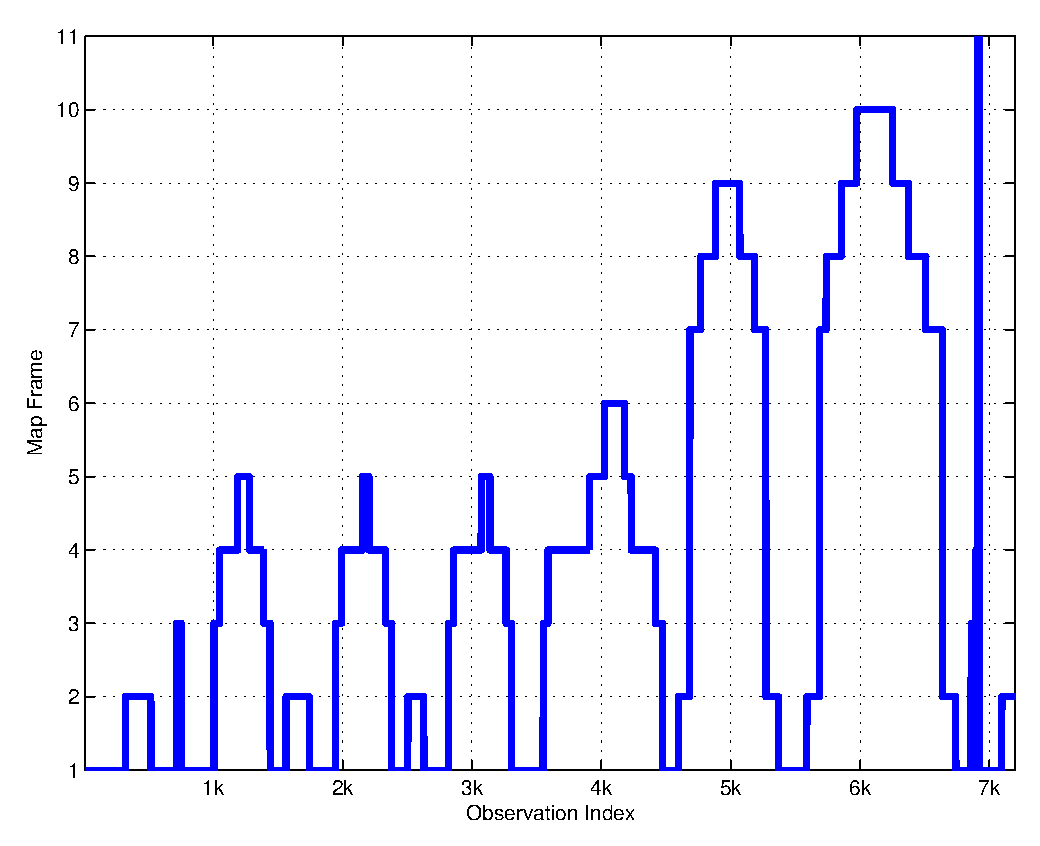
\includegraphics[width=10cm]{Pics/trees_odo_100p}
  }


  \caption{Laser outdoors: Map of corners (100 particles)} %map 33
  \label{fig:trees_map_100p}
\end{figure}

\begin{figure}[htbp]
  \centering
  \subfigure[Projection of the HTSLAM map in the reference frame of map 1.]{
    \includegraphics[width=15cm]{Pics/trees_map_300p}
  }
  \subfigure[Topological path of the robot.]{
    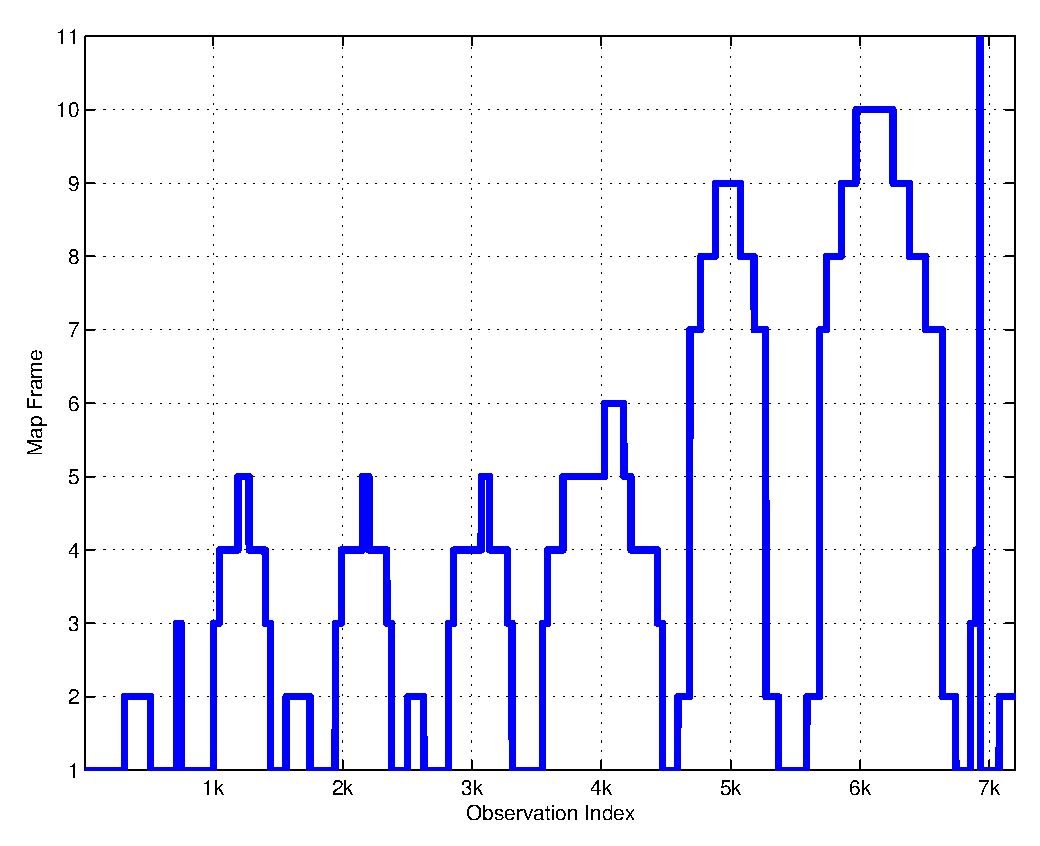
\includegraphics[width=10cm]{Pics/trees_odo_300p}
  }


  \caption{Laser outdoors: Map of corners (300 particles)} %map 33
  \label{fig:trees_map_300p}
\end{figure}

\begin{figure}[htbp]
  \centering
  \subfigure[100 particles]{
    \includegraphics[width=10cm]{Pics/trees_odo_all_100p}
  }
  \subfigure[300 particles]{
    \includegraphics[width=10cm]{Pics/trees_odo_all_300p}
  }
  \caption{Laser outdoors: Global Path over 100 test runs.}
  \label{fig:trees_odo_all}
\end{figure}







% LocalWords:  Odometry HTSLAM Pics odo EKF XR holonomic matlab ACFR FastSLAM
% LocalWords:  Kalman RSISE ANU Jacobian Jacobians odometry Ackerman RMS priori
% LocalWords:  Gaussians
